\documentclass[acmtog]{acmart}
\usepackage{graphicx}
\usepackage{subfigure}
\usepackage{natbib}
\usepackage{listings}
\usepackage{bm}
\usepackage{amsmath}
\usepackage{algorithm, algpseudocode, hyperref}

\definecolor{blve}{rgb}{0.3372549 , 0.61176471, 0.83921569}
\definecolor{gr33n}{rgb}{0.29019608, 0.7372549, 0.64705882}
\makeatletter
\lst@InstallKeywords k{class}{classstyle}\slshape{classstyle}{}ld
\makeatother
\lstset{language=C++,
	basicstyle=\ttfamily,
	keywordstyle=\color{blve}\ttfamily,
	stringstyle=\color{red}\ttfamily,
	commentstyle=\color{magenta}\ttfamily,
	morecomment=[l][\color{magenta}]{\#},
	classstyle = \bfseries\color{gr33n}, 
	tabsize=2
}
\lstset{basicstyle=\ttfamily}
\newcommand{\code}[1]{\texttt{\color{magenta}{#1}}} % for inline code

% Title portion
\title{{Assignment 2 : Geometric Modeling}} 

\author{Name:\quad hidden  \\ student number:\ hidden
\\email:\quad hidden@shanghaitech.edu.cn}

% Document starts
\begin{document}
\maketitle

\vspace*{2 ex}

\section{Introduction}
In this assignment, the following things are done:
\begin{enumerate}
	\item Camera control and Phong shading (same as the last assignment)

	\item Bezier curve and bezier surface
	
	\begin{itemize}
		\item Evalauate the position of any point on a Bezier curve
		\item Construct a bezier surface from a set of control points
		\item Read in \code{.bzs} files which contains a bunch of control points and render the corresponding multiple bezier surfaces
	\end{itemize}

	\item B-spline curve and B-spline surface
	
	\begin{itemize}
		\item Construct a B-spline curve
		\item Construct a B-spline surface from a set of control points, and render it.
	\end{itemize}

	\item Adaptive mesh generation
	\begin{itemize}
		\item In parameter space, adaptively divide the line into serveral segments, and then construct a Bezier curve from the control points. 
		\item Read in \code{.bzs} files and render the bezier surfaces with adaptive mesh.
	\end{itemize}
\end{enumerate}


\section{Implementation Details}

\subsection{Camera Control and Phong lighting model}

The camera control is the same as the last assignment, except that polygon mode control is added. Basically: 

\begin{itemize}
	\item Use \code{WASD} to move the camera upward, left, downward and right.
	\item Use \code{RF} to move the camera forward and backward.
	\item Use mouse to move camera location.
	\item Use \code{O} to apply \code{glPolygonMode  GL\_FILL} to render the filled polygon.
	\item Use \code{P} to apply \code{glPolygonMode GL\_LINE} to render the wireframe, which can help us take a look at the mesh structure precisely.
\end{itemize}

The Phong lighting model implementation and light settings are same as the last assignment, so we will not discuss it here.

\subsection{Bezier Curve}
The Bezier curve is defined by the following equation:
\begin{equation}
\bm{P}(t) = \sum_{i=0}^{n} \bm{P}_i B_{n,i}(t)
\end{equation}
where $B_{n,i}(t)$ is the Bernstein polynomial of degree $n$ and index $i$

To achieve higher precision and efficiency, we will use de Casteljau's algorithm to calculate this. The algorithm is as follows:

Suppose there are $n+1$ control points with a real number $t$ ($t$ is between $0$ and $1$), then 

\begin{algorithm}
	\caption{De Casteljau's algorithm}
	\begin{algorithmic}[1]
		\Procedure{DeCasteljau}{$\bm{P}_0, \bm{P}_1, \cdots, \bm{P}_n, t$}
		\State $Q_0 = \bm{P}_0$
		\For{$i = 1$ to $n$}
		\State $Q_i = (1-t)Q_{i-1} + t\bm{P}_i$
		\EndFor
		\State \Return $Q_n$
		\EndProcedure
	\end{algorithmic}
\end{algorithm}

The tangent vector of each point is also calculated in the above process. 

Therefore given a set of control points, we increase $t$ gradually from $0$ to $1$ with step \code{float DIM\_RECIPROCAL = 0.02} and store each result point in \code{std::vector<vec3>}, and we can get a approximated continous curve. 

\subsection{Bezier Surface}

Now that we know how to evaluate a single-dimensional Bezier curve. To evaluate a 2-dimensional Bezier surface, we simply calculate the tensor product of the two single-dimensional curves. 

In detail, the evaluation can be divided into the following steps:

\begin{enumerate}
	\item Evaluate the position of each point on each set of control points along \code{u} direction.
	\item Utilize the evaluated points as a new set of control points, and generate the final point along \code{v} direction. Note that the tangent along \code{v} direction is simutaneously calculated.
	\item Swap \code{u} and \code{v} and repeat the above two steps again. This time we get the same position and the tangent along \code{u} direction. The normal vector is the cross product of the two orthogonal tangent vectors.
\end{enumerate}

After the above process, we have completed the generation of a mesh grid. We know each points' position and normal. In order to render it, we simply divide each quadrilateral into two triangles. Then we bind then to \code{VAO}, \code{VBO} and \code{EBO} and apply Phong lighting model similar to what we did in assignment 1. 

\subsection{Multiple bezier surface and stitching}

In order to render multiple bezier surfaces, we need to be sure it satisfies continuity. 

Since the provided \code{.bzs} files are all already continous, we can simply process them one by one and load them together.

\subsection{B-spline curve}

Given $n+1$ control points $\bm{P}_0, \bm{P}_1, \cdots, \bm{P}_n$ and a knot vector $\bm{K} = (k_0, k_1, \cdots, k_{n+m+1})$, the B-spline curve of degree $p$ at point $u$ is defined by the following equation:
\begin{equation}
	\bm{P}(u) = \sum_{i=0}^{n} \bm{P}_i N_{i,p}(u)
\end{equation}

where $n, m, p$ must satisfy $m = n + p + 1$.

The basis function $N_{i,p}(u)$ is defined by the Cox-de Boor recursion formula:

\begin{equation}
	N_{i,0}(u) = \begin{cases}
		1, & k_i \leq u < k_{i+1} \\
		0, & \text{otherwise}
	\end{cases}			
\end{equation}

\begin{equation}
	N_{i,p}(u) = \frac{u-k_i}{k_{i+p}-k_i}N_{i,p-1}(u) + \frac{k_{i+p+1}-u}{k_{i+p+1}-k_{i+1}}N_{i+1,p-1}(u)
\end{equation}

Since $N_{i,p}$ is non-zero only when $k_i \leq u < k_{i+p+1}$, at most $p+1$ degree-p-based functions are nonzero. Therefore, the B-spline curve can be approximated by the following algorithm:

\[
	Q_i = (1-a_i) P_{i-1} + a_i P_i	
\]
where $a_i$ is \[
	a_i = \frac{u-k_i}{k_{i+p+1}-k_i} 	
\] for $k-p+1\leq i \leq k$

The $Q_i$ is the new control point calculated by $P_{i-1}$ and $P_i$. 




% The new control points are stored in a new vector $\bm{Q}$, and the new knot vector is calculated by the following formula:



If a knot $u$ is inserted repeatedly until its multiplicity is $p$, the last generated new control point is exactly the result $P(u)$. Therefore if $u$ lies in the interval $[k_i, k_{i+1})$, the new control point $Q_i$ is the result $P(u)$.



\subsection{B-spline surface}

The construction of B-spline surface is almost the same as the Bezier surface. The only difference is that we need to calculate the B-spline basis function instead of the Bernstein polynomial. Therefore we won't go into details here. Refer to subsection 2.2 (Bezier surface) for detailed explanations.


\subsection{Adaptive mesh generation}

In the previous sections, we have already known how to generate a mesh grid. However, the sample points along $u$ and $v$ directions have fixed density, which is defined by \code{float DIM\_RECIPROCAL = 0.02} in the implementation. There might be too many unnecessary points on an almost straight curve, or too few points on a winding curve. We can solve this problem by generating an adaptive mesh, letting the number of sample points varying according to the curvature of the curve. 

First let's focus on the Bezier curve. We use divide and conquer to divide the curve recursively until the curvature of the curve is small enough. To demonstrate the algorithm, we take a look at the picture below (the picture is from \href{https://agg.sourceforge.net/antigrain.com/research/adaptive_bezier/index.html}{sourceforge}):

\begin{center}
	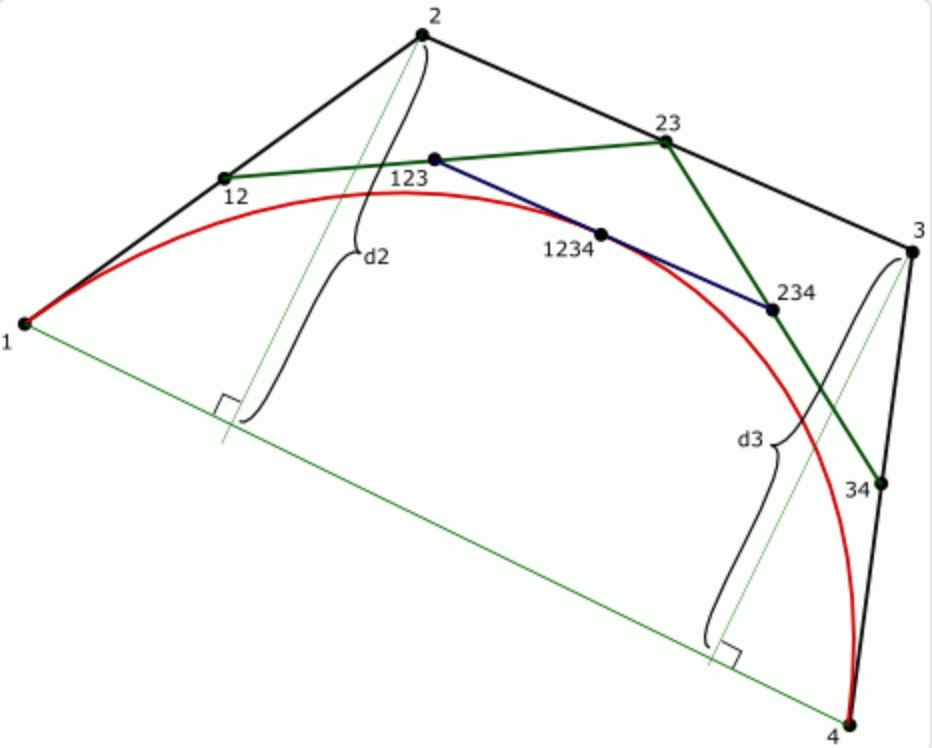
\includegraphics[width=0.4\textwidth]{./images/adaptive-bezier.jpg}
\end{center}

Suppose there are 4 control points, namely \code{p1}, \code{p2}, \code{p3} and \code{p4}. We first calculate the middle point \code{p12}, \code{p23} and \code{p34}. Similar for \code{p123} and \code{p234}, and finally \code{p1234}. 

We will check if the distance between \code{p1234} and the line segment between \code{p1} and \code{p4} is small enough. If it is, we will simply add \code{p1234} to the result vector, because the curve is straight enough so that we can use a straight line to simulate it. Otherwise, we will divide the curve into two parts and recursively call the function, for densier division.

The critical part is that, how do we check the `distance' is small enough or the segment is flat enough. To do that, we first calculate distance from \code{p2} to the line \code{p1p4}, namely \code{d2} as shown in the picture. Similar for the distance between \code{d3} and \code{p1p4} called \code{d3}. Then we check whether \[
	d_2 + d_3 \leq \epsilon \cdot d_{1,4}	
\]
to determine the flatness. The $\epsilon$ is a tolerance paramter, that is, higher value means higher tolerance and fewer points will be generated, and vice versa. 

Then, given 4 control points, we use the following code to adaptively divide the line: 

% \newpage

\begin{algorithm}
	\caption{Recursive subdivision}
	\begin{algorithmic}[1]
		\Procedure{division}{$\bm{P}_1, \bm{P}_2, \bm{P}_3, \bm{P}_4$} \Return {sample points}
		\If{recursion level is too deep} 
			\State \Return \textbf{Points}
		\EndIf

		\State \textbf{calculate} mid points $p12, p23, p34$, $p123, p234$,$p1234$

		\State \textbf{calculate} distance $d2$ and $d3$

		\If{$d2 + d3$ $\leq$ $tolerance * d14$}
			\State Add the midpoint $p1234$ to \textbf{Points}
			\State \Return \textbf{Points}
		\EndIf

		\State Division($\bm{P}_1, \bm{P}_{12}, \bm{P}_{123}, \bm{P}_{1234}$)

		\State Division($\bm{P}_{1234}, \bm{P}_{234}, \bm{P}_{34}, \bm{P}_4$)

		\EndProcedure
	\end{algorithmic}
\end{algorithm}


After that we can use the procedure to help us generate points for a Bezier surface. Suppose we have a $4\times 4$ control point matrix, then the adaptive mesh generation is done with the following steps: 

\begin{enumerate}
	\item Apply the above division process to each set of control points along \code{u} direction and store the generated sample points. 
	\item Divide [0,1] into ten segments. For each segment, taking [0.2, 0.3] as an example, apply De Casteljau's algorithm to get the position, and check how many points lies in the corresponding interval.
	\item Repeat the above step for each row of adaptive sample points and take the max number of points \code{n}. Then divide the interval [0.2, 0.3] into \code{n} small segments.
	\item For \code{v} direction, apply similar process and obtain the points on \code{v} direction.
	\item Similar as the Bezier surface generation, generate the triangles and bind \code{VAO, VBO, EBO}.
\end{enumerate}

In this way, we can avoid the complex trianglization, since what we have generated is also a quadrangle-shaped mesh, and the object generation is almost the same.


\newpage

\section{Results}

\subsection{Bezier surface (uniform single bezier surface)}

Below is a single bezier surface with specified 4*4 control points matrix.

\begin{center}
	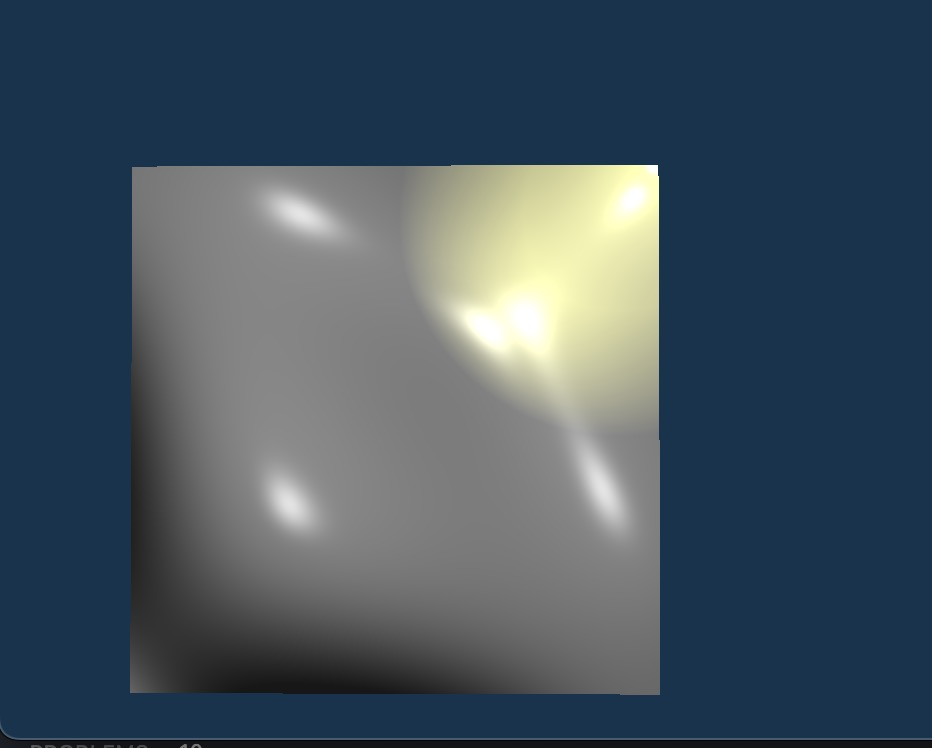
\includegraphics[width=0.4\textwidth]{./images/bezier-surface.jpg}
\end{center}

\subsection{Multiple bezier surface (tea set)}

Below is the rendered result of \code{assets/tea.bzs} file. The file contains multiple continous bezier surfaces' control points, which forms the tea set. 

\begin{center}
	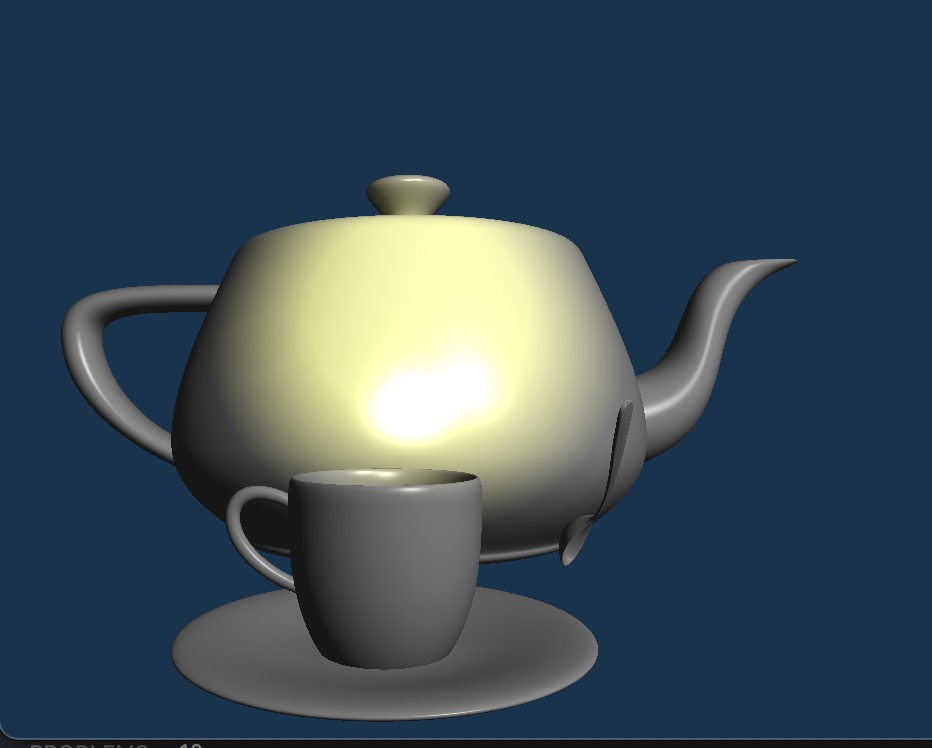
\includegraphics[width=0.4\textwidth]{./images/bezier-tea-set.jpg}
\end{center}

\subsection{B-spline surface (uniform single b-spline surface)}

\begin{center}
	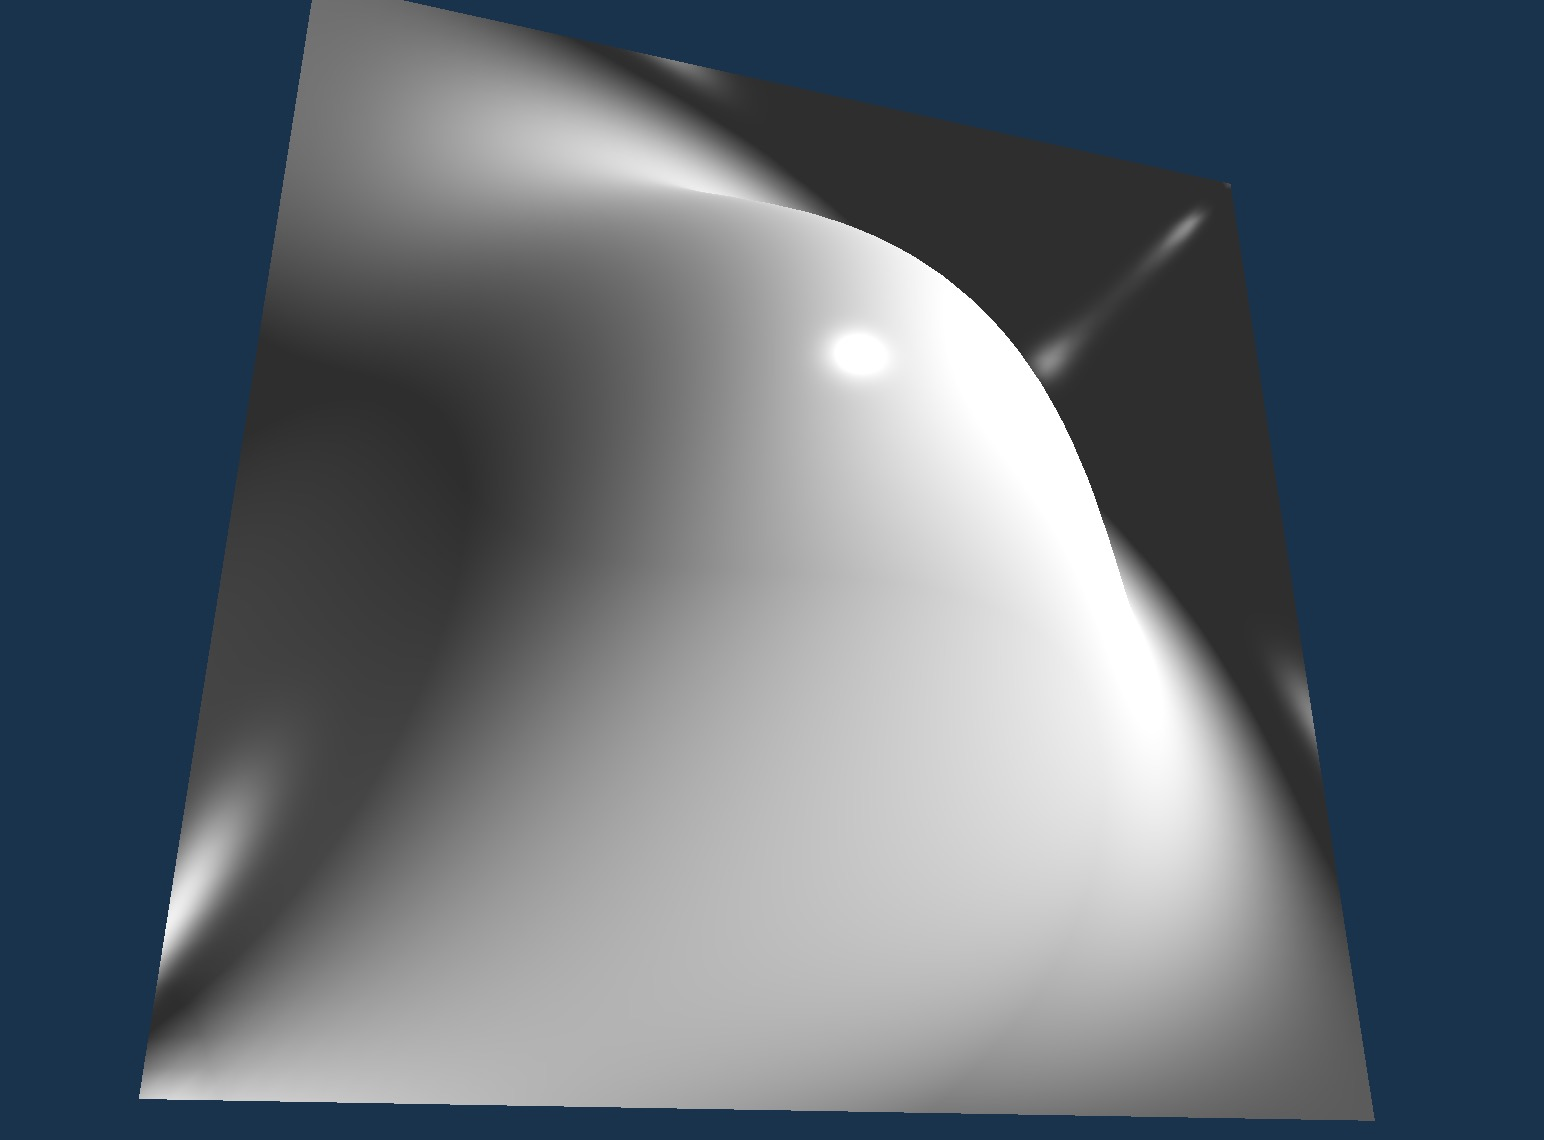
\includegraphics[width=0.4\textwidth]{./images/bspline.jpg}
\end{center}

% \newpage

\subsection{Adaptive Mesh (adaptive single bezier surface)}

% By comparing the same bezier surface generated in uniform and adaptive, we can clearly see the difference.

\begin{center}
	Adaptive single bezier surface
	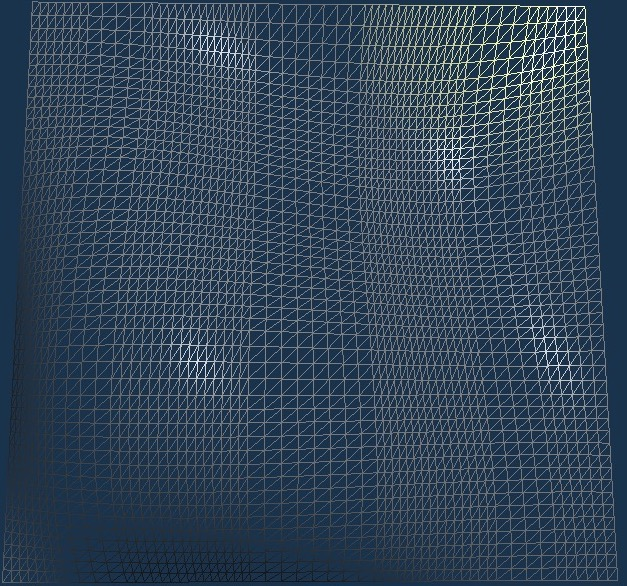
\includegraphics[width=0.4\textwidth]{images/adaptive-single-1.jpg}
\end{center}

\begin{center}
	Uniform bezier surface
	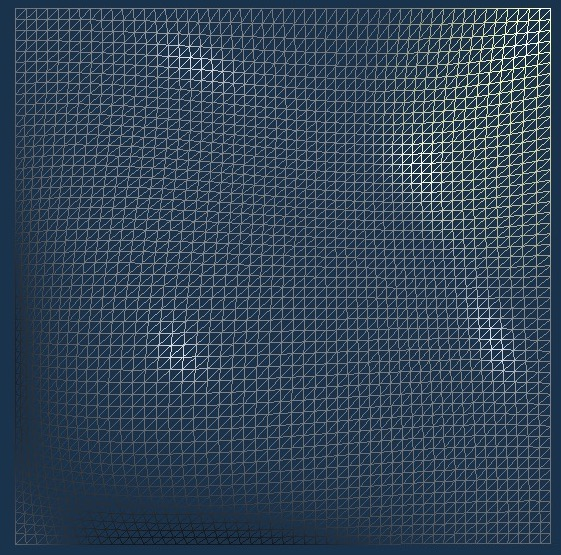
\includegraphics[width=0.4\textwidth]{images/not-adaptive-single-1.jpg}
\end{center}

\newpage

\subsection{Adaptive Mesh (adaptive multiple bezier surface)}

From the picture shown below, with adaptive mesh generation, the mesh is denser on the winding part (e.g. the front tea cup) and sparser on the straight part (the rear larger tea set), while without adaptive meshing, the mesh has the same density everywhere.

\begin{center}
	Tea set with adaptive meshing
	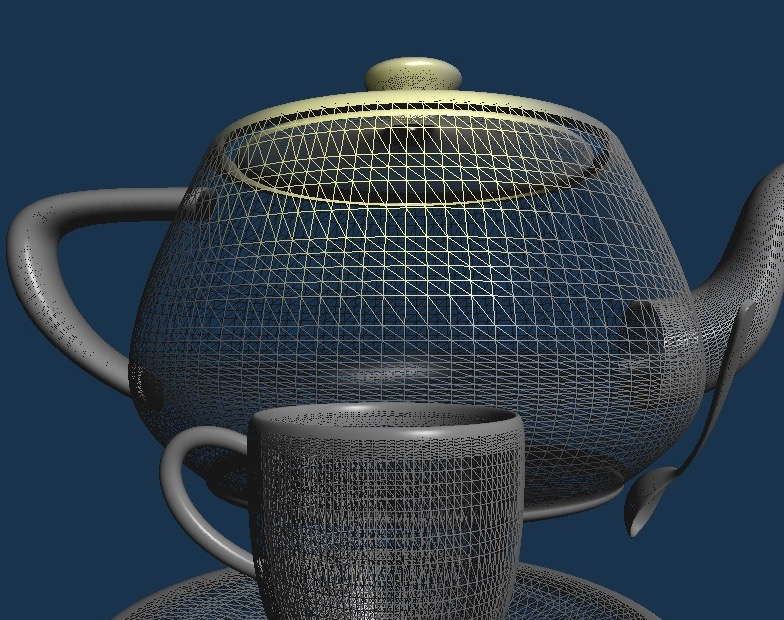
\includegraphics[width=0.4\textwidth]{images/adaptive-1.jpg}
\end{center}

\begin{center}
	Tea set without adaptive meshing (uniform meshing)
	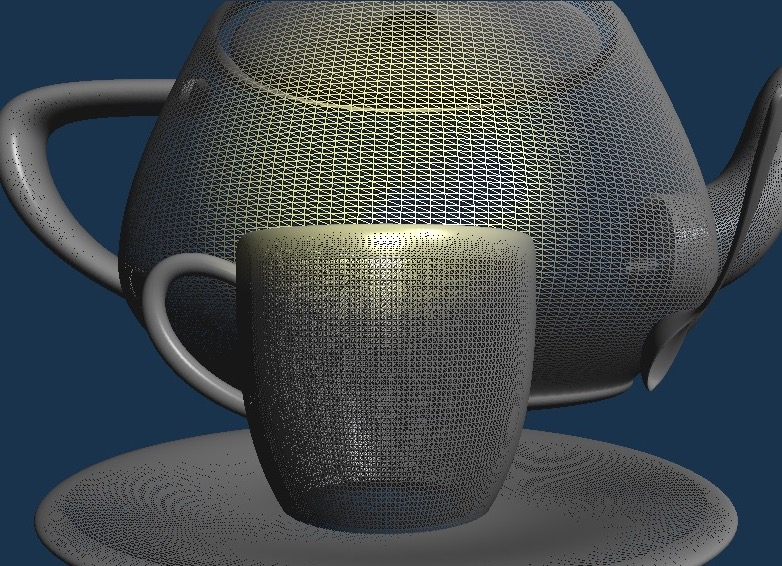
\includegraphics[width=0.4\textwidth]{images/not-adaptive-1.jpg}
\end{center}

% \begin{center}
% 	Tea set with adaptive meshing (detail)
% 	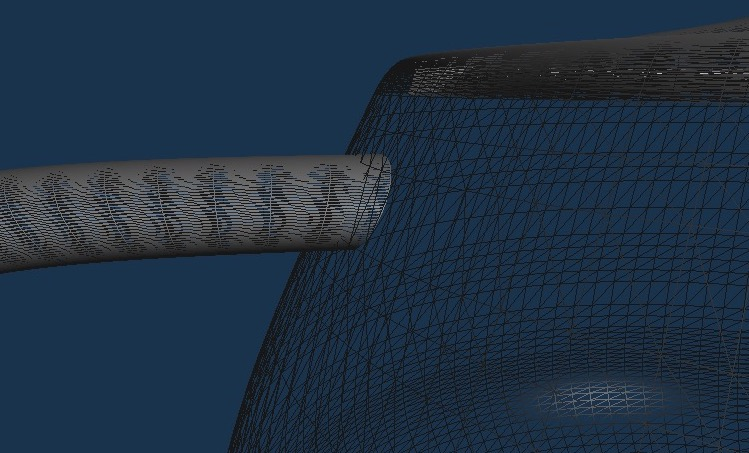
\includegraphics[width=0.4\textwidth]{images/adaptive-2.jpg}
% \end{center}

% \begin{center}
% 	Tea set with uniform meshing (detail)
% 	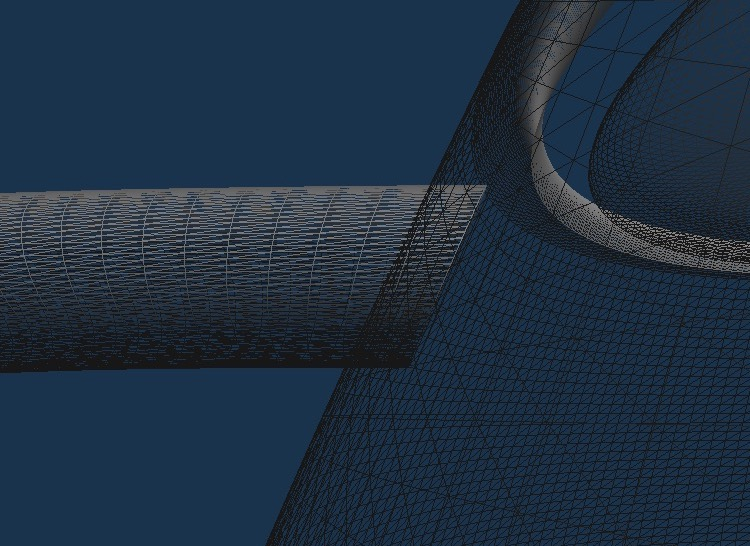
\includegraphics[width=0.4\textwidth]{images/not-adaptive-2.jpg}
% \end{center}

% pictures should be in
\end{document}
